\appendix

\addcontentsline{toc}{part}{Annexes}

\part*{Annexes}

\chapter{Le fonds Araucania}
\begin{figure}
	    \centering
    	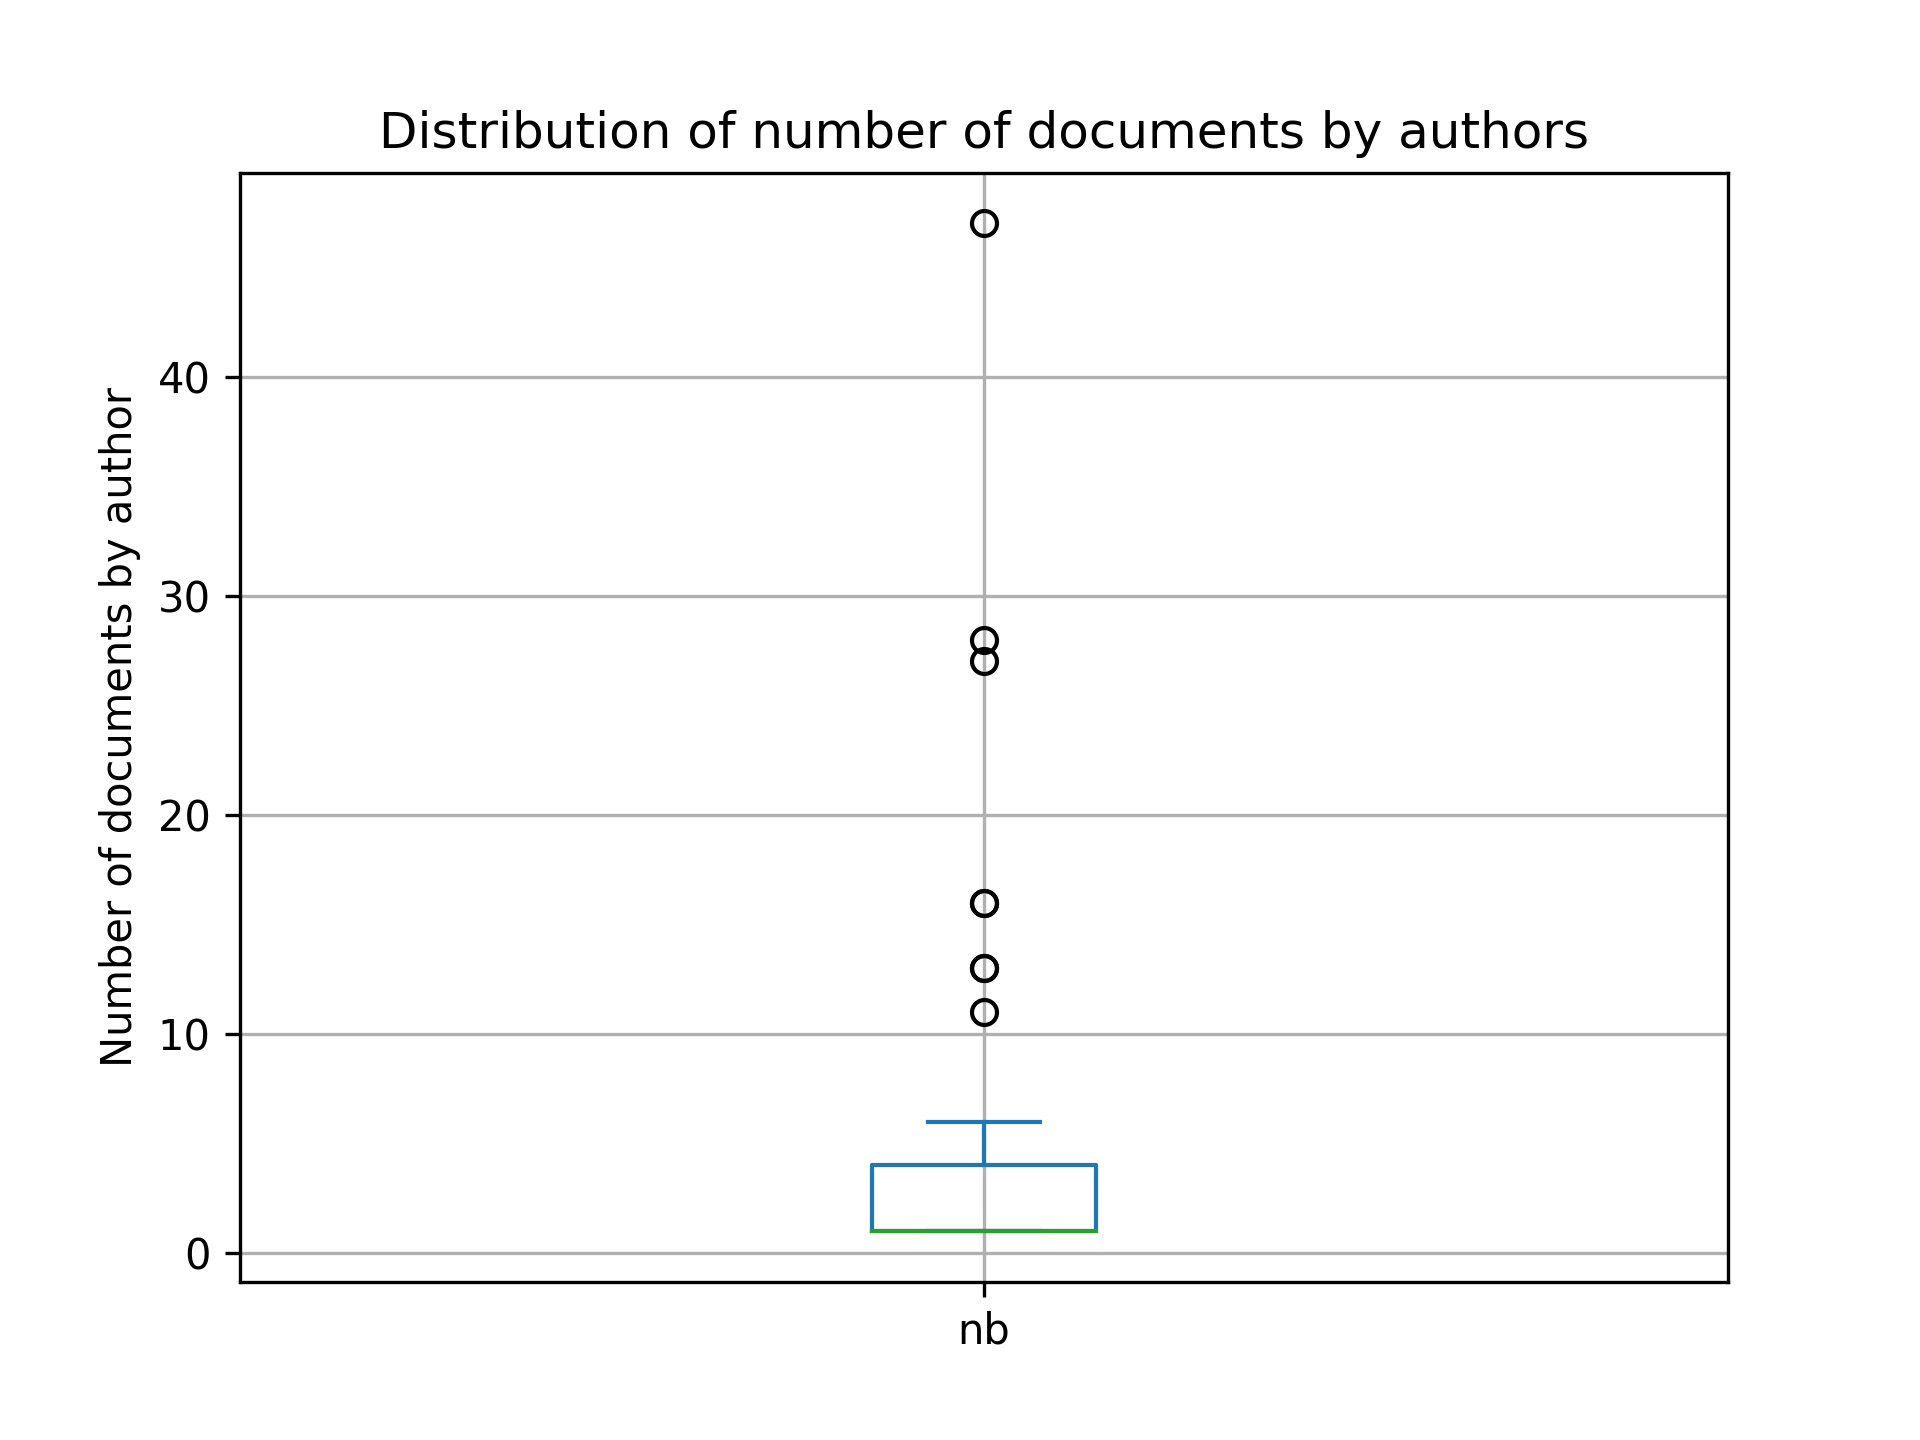
\includegraphics[width = 1\textwidth]{annexes/graph/author_distribution.png}
    	\caption{Distribution du nombres de documents par auteurs}
    	\label{fig:author_distribution}
    	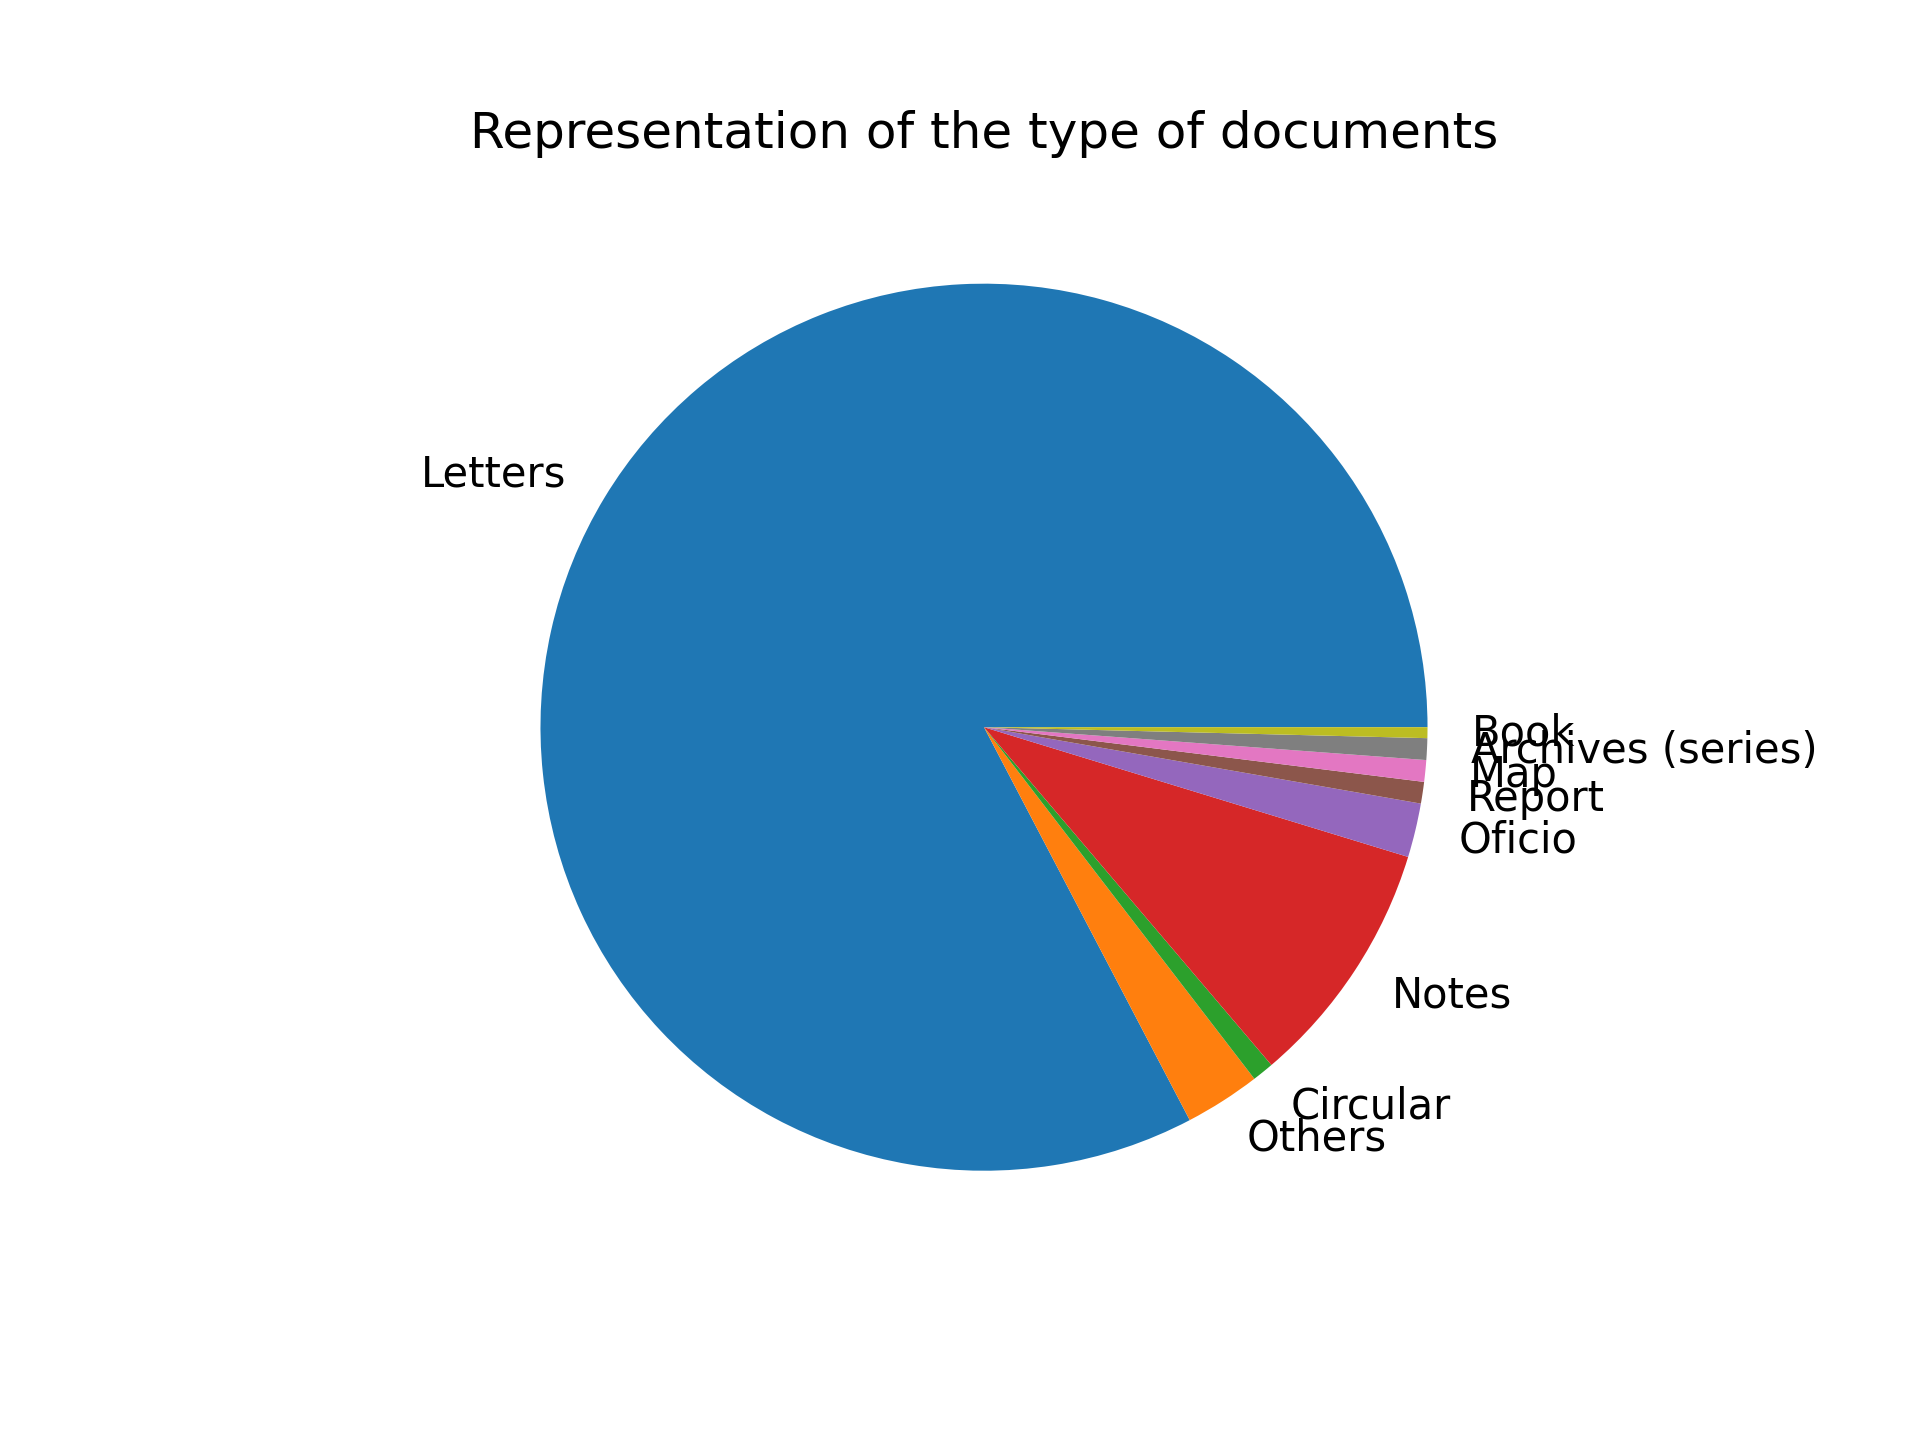
\includegraphics[width = 0.9\textwidth]{annexes/graph/percent_type.png}
    	\caption{Représentation des documents selon leur nature}
    	\label{fig:percent_type}
\end{figure}
\begin{figure}
    \centering
    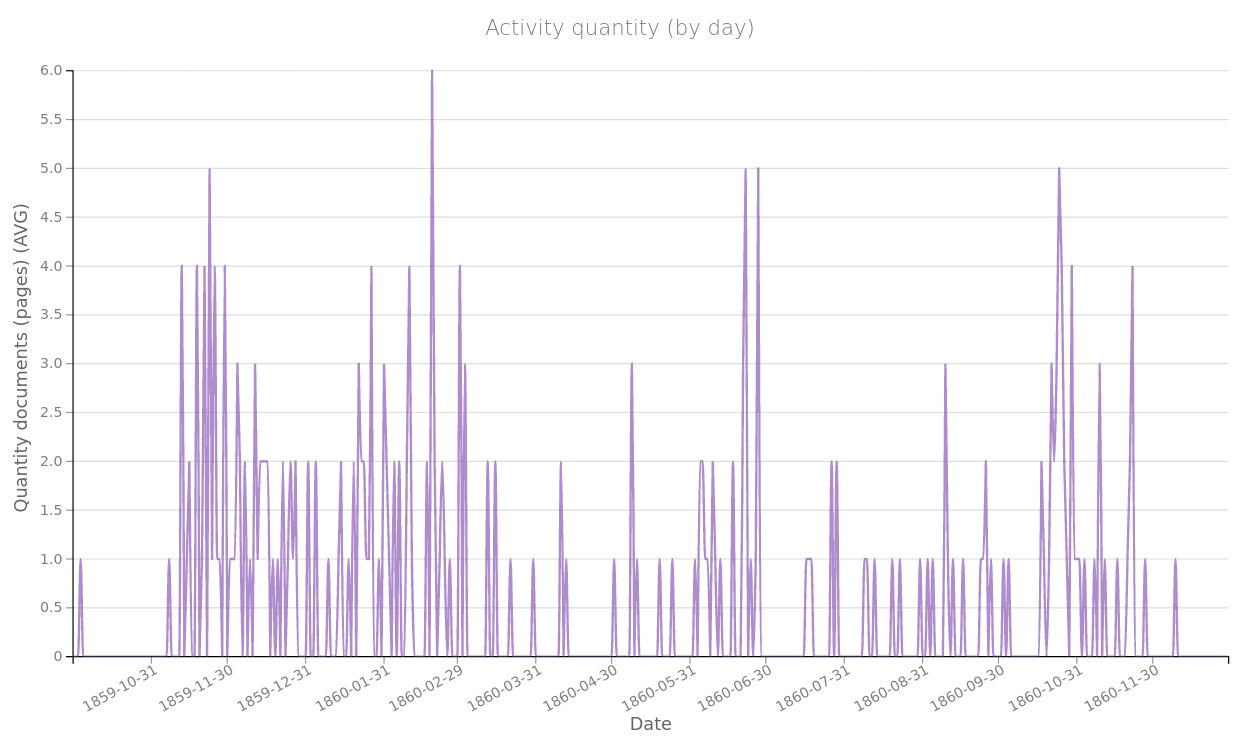
\includegraphics[width = 1\textwidth]{annexes/graph/activity_quantity_day.png}
    \caption{Activités documentaires sur les années 1859-1860 (par jours)}
    \label{fig:day_activities}
    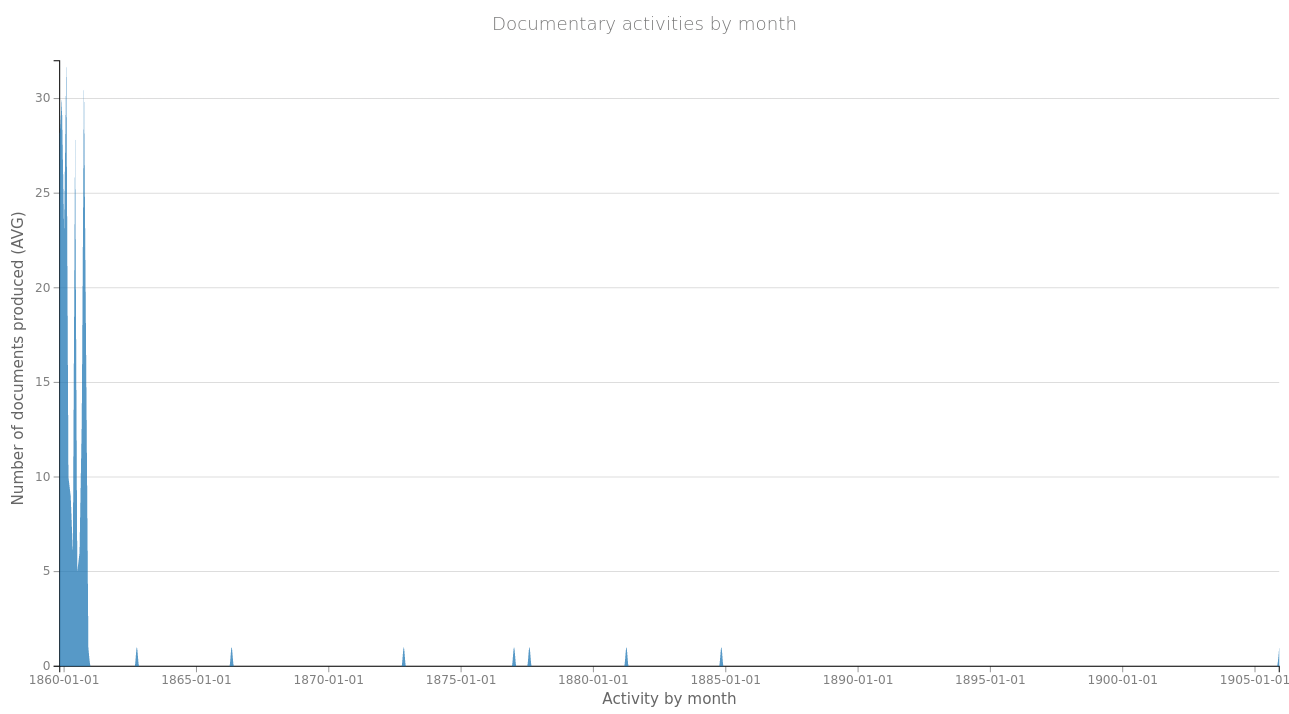
\includegraphics[width = 1\textwidth]{annexes/graph/archives_activity_month.png}
    \caption{Activités documentaires (par mois)}
    \label{fig:month_activities}
\end{figure}

\begin{figure}
     \centering
     \begin{subfigure}[b]{0.8\textwidth}
         \centering
         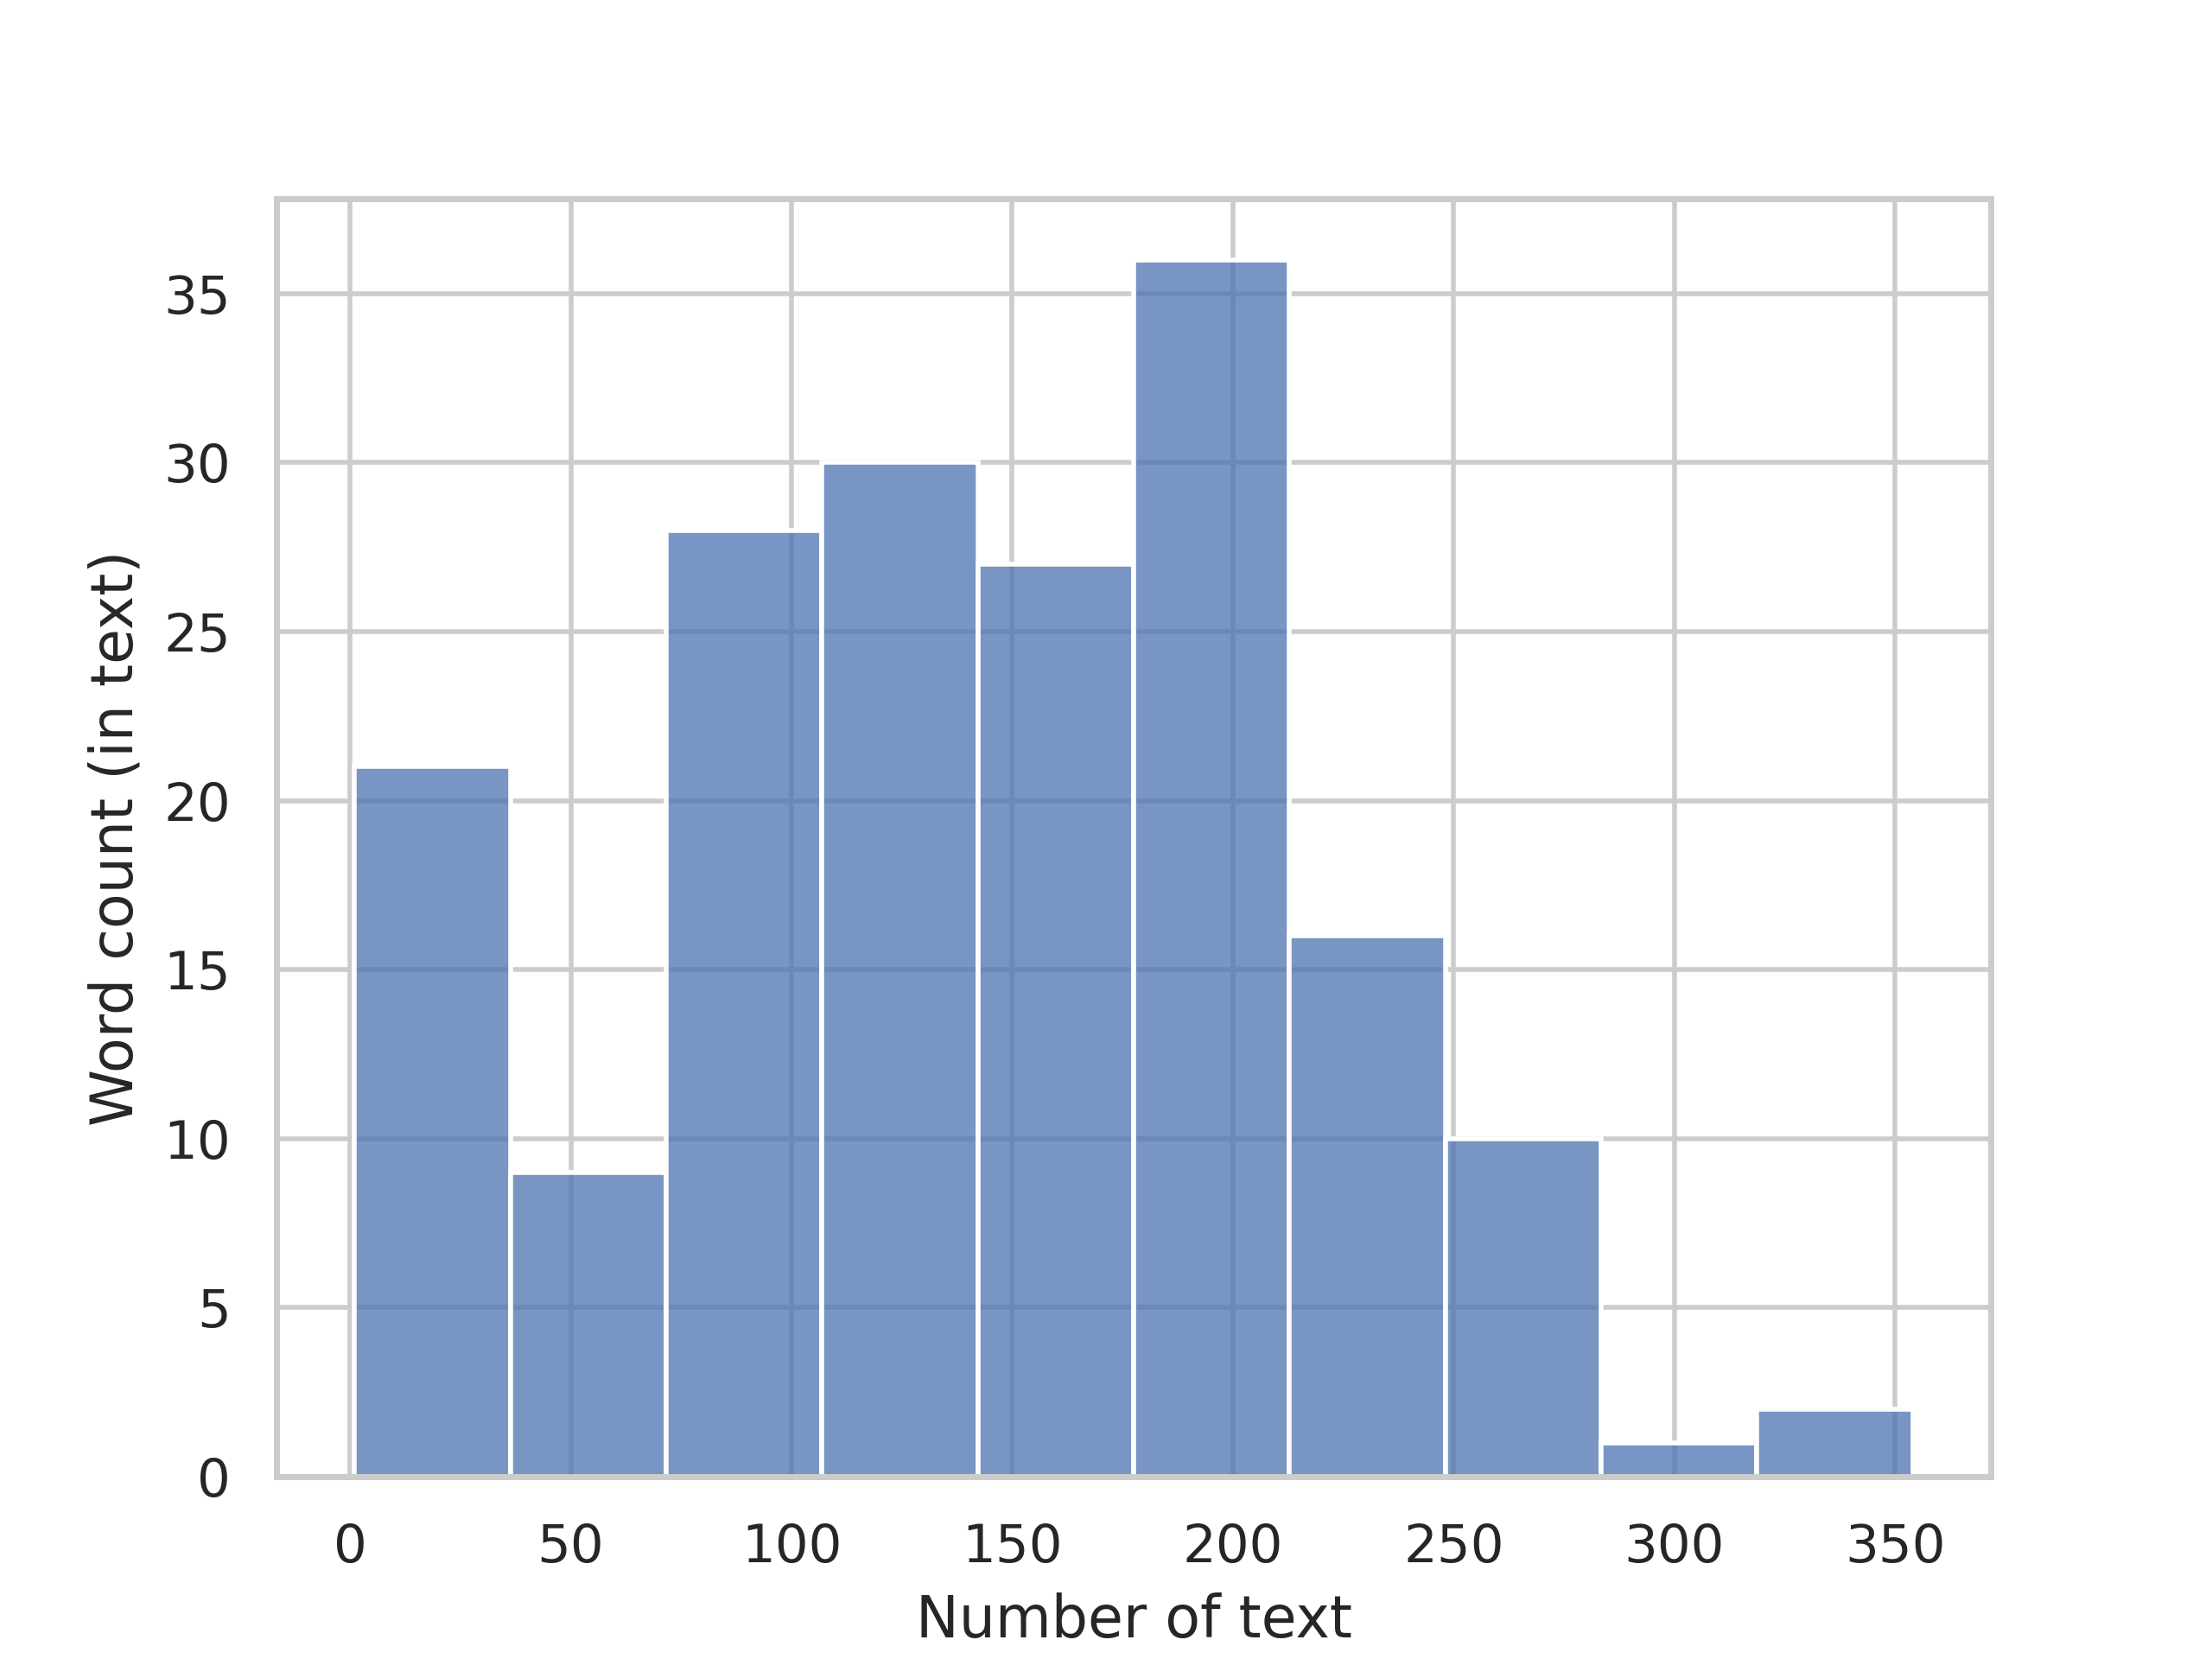
\includegraphics[width=\textwidth]{annexes/graph/histo_word_total.png}
         \caption{Par pages}
         \label{fig:histo_word_total}
     \end{subfigure}
     \hfill
     \begin{subfigure}[b]{0.8\textwidth}
         \centering
         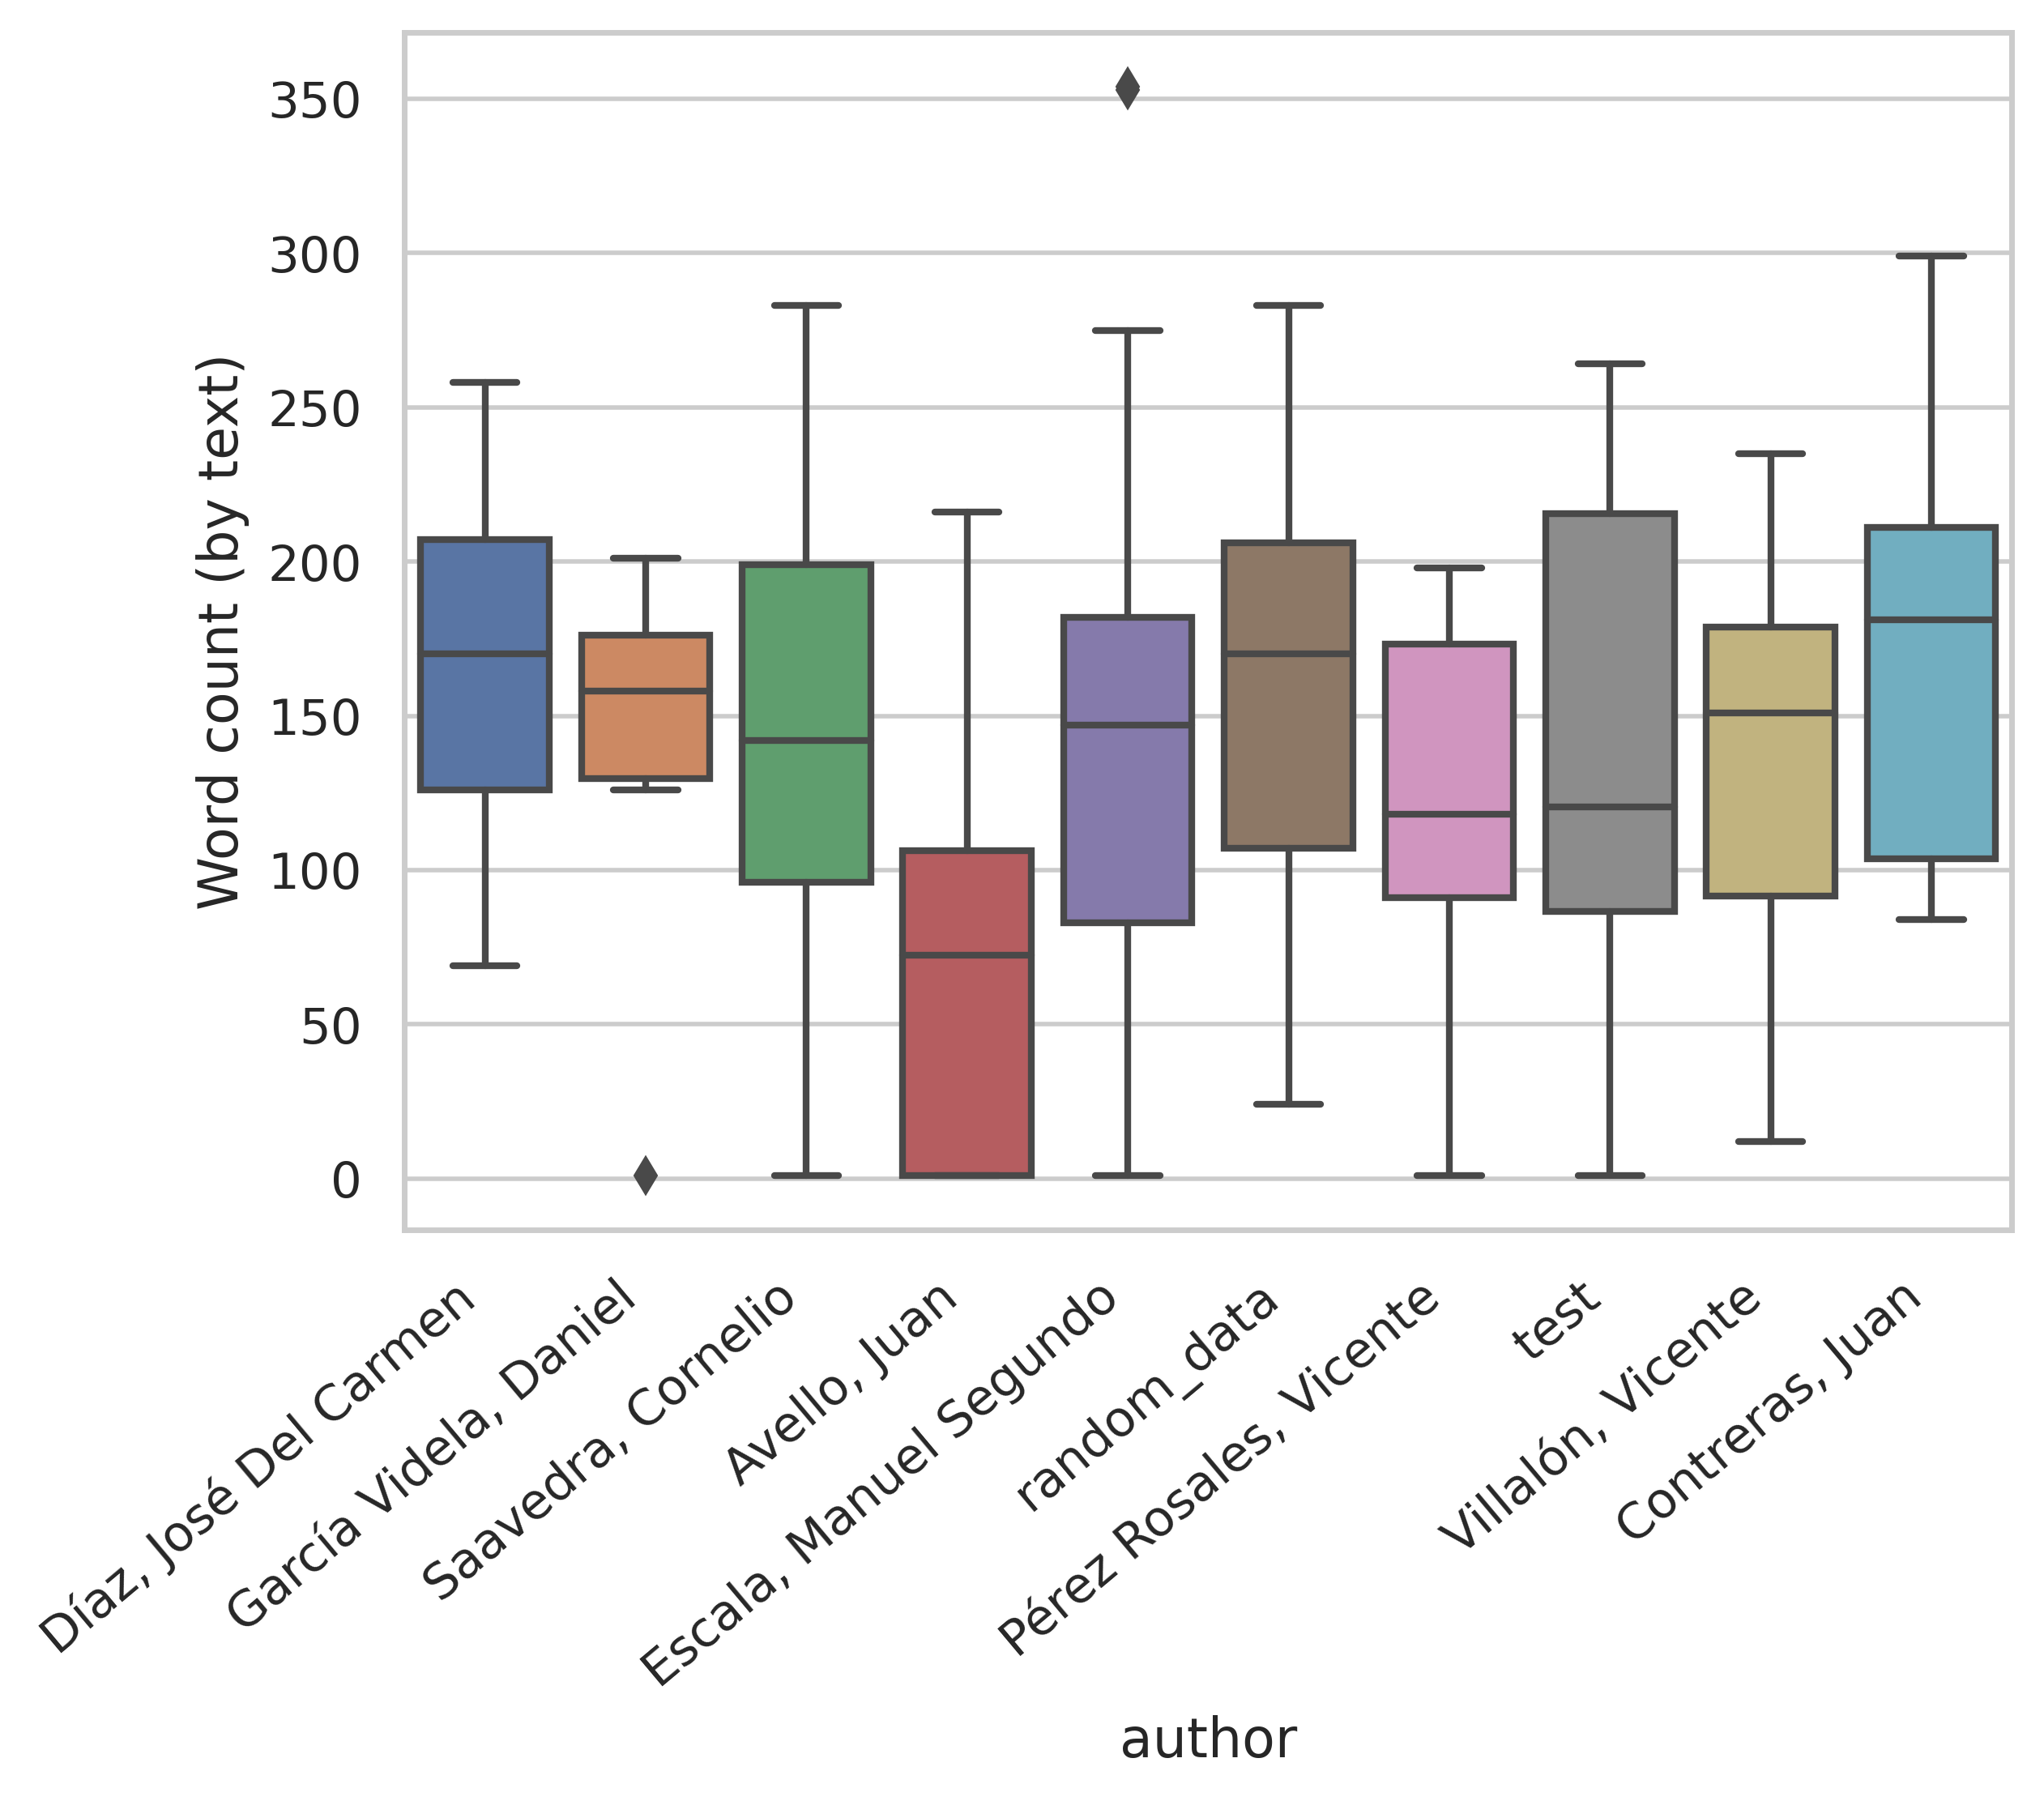
\includegraphics[width=\textwidth]{annexes/graph/boxtop_word.png}
         \caption{Par auteurs}
         \label{fig:boxtop_word}
     \end{subfigure}
     \caption{Distribution des mots}
    \label{fig:three graphs}
\end{figure}

\chapter{Automatisation d'une conversion de format d'image}
\chaptermark{Conversion de format d'image}
\begin{listing}
	        \begin{minted}{shell}
	        #!/bin/bash

                FOLDER=~/Bureau/data/jpg 
                ERROR="$FOLDER/error.txt"
                
                if ! [[ -d "$FOLDER" ]]|| ! [[ -e $ERROR ]]
                then
                	mkdir -p $FOLDER
                	touch $ERROR
                else
                    rm -f "$FOLDER/*.jpg"
                fi
                
                for img in "$PWD"/*.tif; do 
                    filename="$(basename "${img%.tif}")"
                    convert "$img" "$FOLDER/$filename.jpg"
                done 2>> $ERROR
	        \end{minted}
        	\caption{Script de conversion d'images TIFF vers le format JPG}
        	\label{code:shell_img}
\end{listing}

\chapter{Exemple de binarisation et de seuillage d'une image}
\chaptermark{}
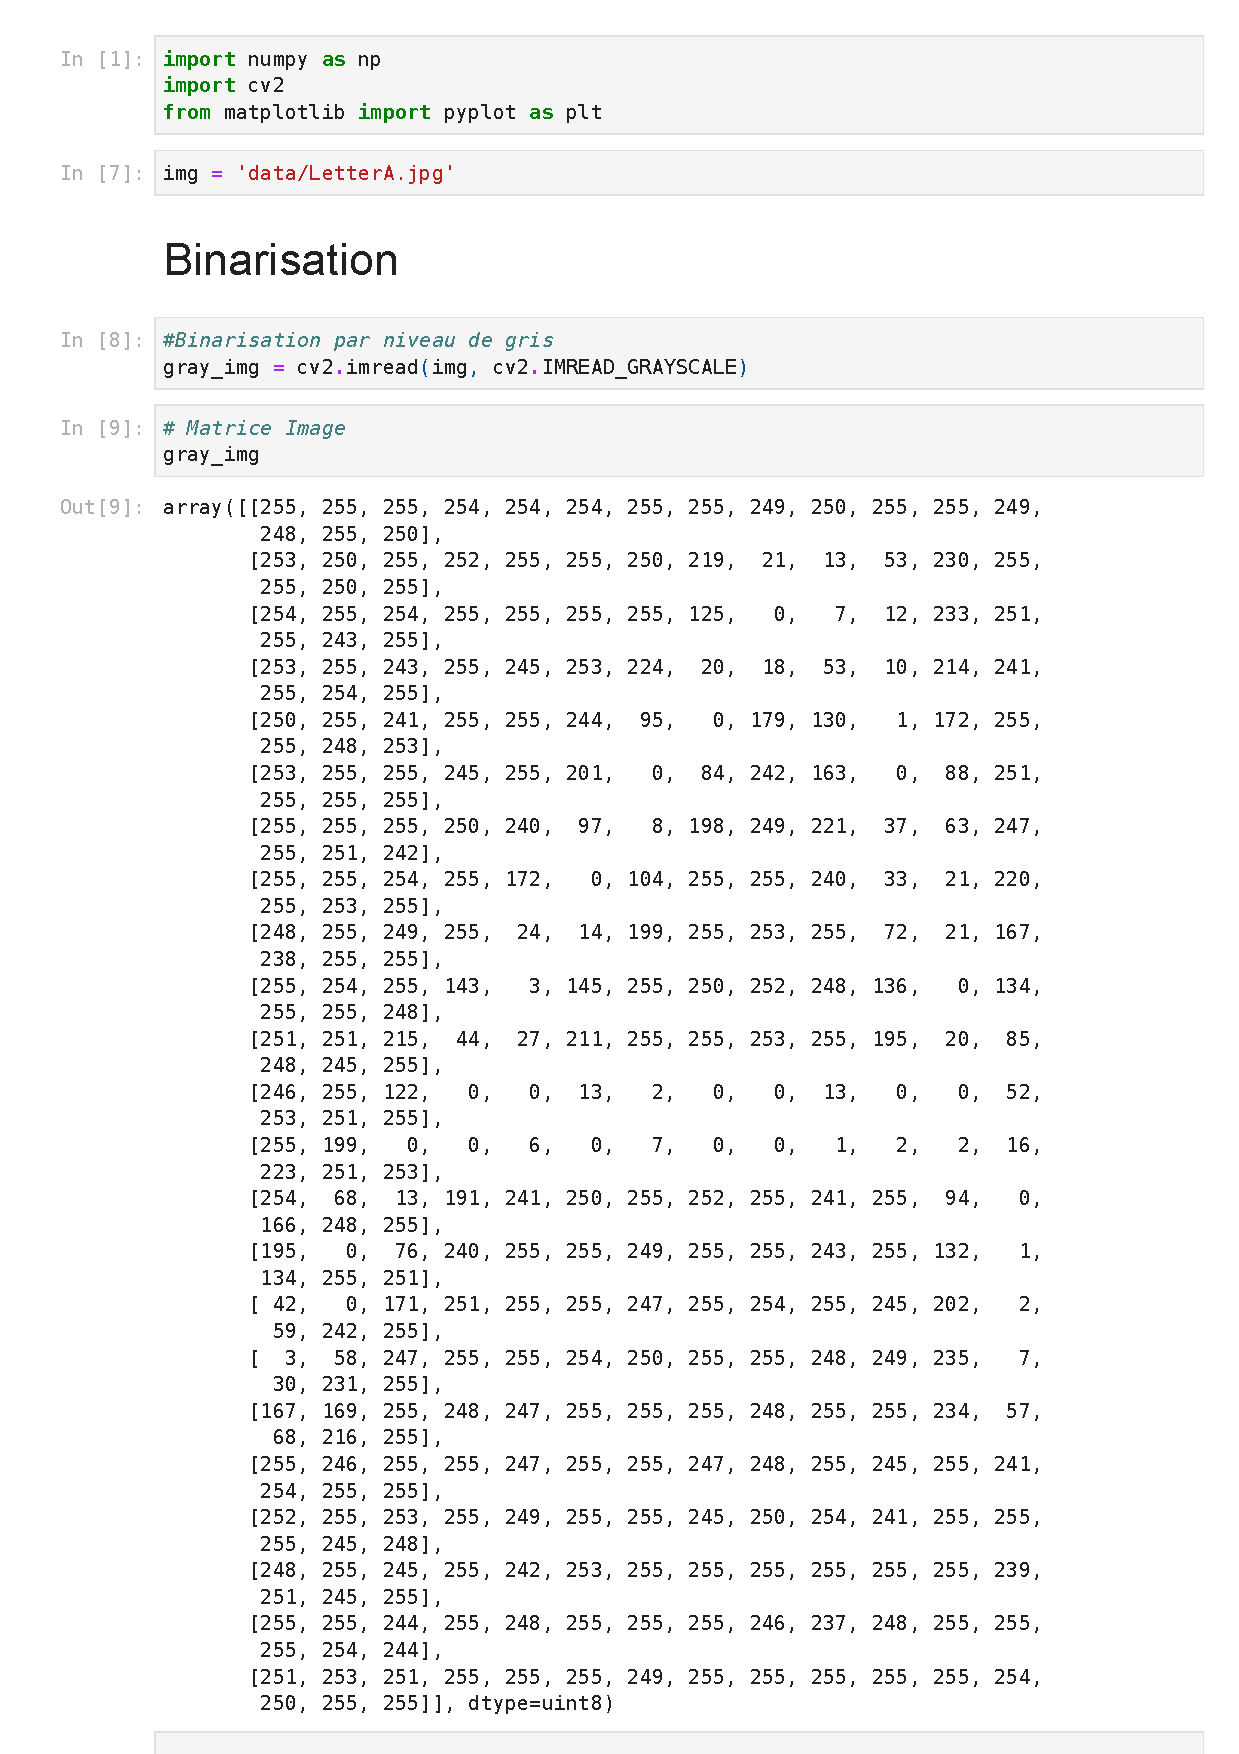
\includepdf[pages=-, pagecommand={}\label{code:traitement_image}]{annexes/pdf/traitement_image_HTR.pdf}

\chapter{Entraînement d'un modèle HTR avec Kraken}

\begin{listing}[h]
\centering
	        \begin{minted}{shell}
	        ketos train --augment --workers 8 -d cuda:0 -f binary --min-epochs 20 -w 0 -s '[1,120,0,1Cr3,13,32 Do0.1,2 Mp2,2 Cr3,13,32 Do0.1,2 Mp2,2 Cr3,9,64 Do0.1,2 Mp2,2 Cr3,9,64 Do0.1,2 S1(1x0)1,3 Lbx200 Do0.1,2 Lbx200 Do.1,2 Lbx200 Do]' --optimizer Adam -B 20 -r 0.0001 dataset.arrow > train_skratch.txt
	        \end{minted}
        	\caption{Commande shell d'entraînement selon la méthode \textit{skratch}}
        	\label{code:skratch}
\end{listing}

\begin{listing}[h]
    \centering
	        \begin{minted}{shell}
	        ketos train -f binary --augment -B 20 -d cuda:0 -o araucania_finetuning_McFrench --resize both --load HTR-United-Manu_McFrench.mlmodel dataset.arrow --lrate 0.0001 --workers 8 > train_finetuning.txt
	        \end{minted}
        	\caption{Commande shell d'entraînement selon la méthode \textit{finetuning}}
        	\label{code:finetuning}
\end{listing}

\begin{listing}[h]
            \centering
	        \begin{minted}{shell}
	        ketos segtrain --augment -d cuda:0 -s '[1,1800,0,3 Cr7,7,64,2,2 Gn32 Cr3,3,128,2,2 Gn32 Cr3,3,128 Gn32 Cr3,3,256 Gn32 Cr3,3,256 Gn32 Lbx32 Lby32 Cr1,1,32 Gn32 Lby32 Lbx32]' -f alto -bl data/**/*.xml -r 0.0001 --resize both --optimizer Adam -i models/blla.mlmodel --merge-baselines DefaultLine:default --merge-regions MainZone:text > segtrain.txt  
	        \end{minted}
        	\caption{Commande shell d'entraînement selon la méthode \textit{finetuning} d'un modèle de segmentation}
        	\label{code:segment}
\end{listing}

\chapter{Exemple de fichier XML-TEI : AH0299}
\chaptermark{Exemple de fichier XML-TEI}

\begin{minted}{xml}
<?xml version='1.0' encoding='UTF-8'?>
<TEI xmlns="http://www.tei-c.org/ns/1.0">
  <teiHeader>
    <fileDesc>
      <titleStmt>
        <title>Carta del 10 de junio de 1860 de Cornelio Saavedra a Mauricio Barbosa</title>
        <author>Saavedra, Cornelio</author>
        <editor>
          <orgName>Archivo Central Andres Bello</orgName>
        </editor>
      </titleStmt>
      <editionStmt>
        <respStmt>
          <resp xml:id="DirSc">Scientific Director of the edition</resp>
          <persName>
            <forename>Alessandro</forename>
            <surname>Chiaretti</surname>
            <roleName>Professor and archivist, responsable Área de Información Bibliográfica y Archivística</roleName>
            <affiliation>Archivo Central Andres Bello | Universidad de Chile</affiliation>
          </persName>
        </respStmt>
        <respStmt>
          <resp xml:id="Enc">In charge of digital encoding</resp>
          <persName>
            <forename>Maxime</forename>
            <surname>Humeau</surname>
            <roleName>Student, trainee</roleName>
            <affiliation>Ecole nationale des chartes | PSL</affiliation>
          </persName>
        </respStmt>
      </editionStmt>
      <extent>
        <measure unit="images" n="2"/>
      </extent>
      <publicationStmt>
        <publisher xml:id="ACAB">Archivo Central Andres Bello</publisher>
        <authority>Área de Información Bibliográfica y Archivística</authority>
        <address>
          <country key="CL"/>
          <region>Región Metropolitana</region>
          <settlement type="city">Santiago Centro</settlement>
          <postCode>8320000</postCode>
          <street>Arturo Prat</street>
          <street>#23</street>
        </address>
        <availability status="restricted">
          <licence target="https://creativecommons.org/licenses/by-sa/3.0/deed.fr">Attribution-NonCommercial-ShareAlike 4.0 International (CC BY-NC-SA 4.0)</licence>
          <p>Share — copy and redistribute the material in any medium or format</p>
          <p>Adapt — remix, transform, and build upon the material</p>
          <p>Attribution — You must give appropriate credit, provide a link to the license, and indicate if changes were made. You may do so in any reasonable manner, but not in any way that suggests the licensor endorses you or your use.</p>
          <p>NonCommercial — You may not use the material for commercial purposes.</p>
          <p>ShareAlike — If you remix, transform, or build upon the material, you must distribute your contributions under the same license as the original.</p>
          <p>The license is restricted to the use of XML-TEI files. The exploitation, distribution or publication of the attached images is subject to the approval of the institution. The full rights of the archive are reserved. The request can be made to the following address: &lt;email&gt;archivo.central@uchile.cl&lt;/email&gt;</p>
        </availability>
        <date when-iso="2022-08-15"/>
      </publicationStmt>
      <notesStmt>
        <note>Digital editing done as part of an international internship.</note>
        <note>A first transcription of part of the collection was made in &lt;date when-iso="2014-06"&gt;2014&lt;/date&gt; by &lt;persName&gt;Cecilia del Carmen Ramallo Díaz&lt;/persName&gt;.</note>
        <note>HTR scanning done at Universidad de Chile with kraken engine and the application eScriptorium. The HTR models from the transcript are available at this address &lt;ref target="https://github.com/Proyecto-Ocupacion-Araucania-UChile/model-HTR"&gt;github&lt;/ref&gt;</note>
      </notesStmt>
      <sourceDesc>
        <bibl>
          <series xml:lang="es">
            <title series="s" type="principal">Colección Manuscritos</title>
            <title type="subtitle">Pacificacion de la Araucania</title>
            <respStmt>
              <resp>Classification and conservation by</resp>
              <persName ref="#DirSc">Alessandro Chiaretti</persName>
              <persName xml:id="M_Parra">Marcos Parra</persName>
              <orgName ref="#ACAB">Área de Información Bibliográfica y Archivística</orgName>
            </respStmt>
            <idno type="caja" n="3"/>
            <idno type="id" n="AH0299"/>
            <note>
              <unit type="documents" quantity="255"/>
            </note>
          </series>
        </bibl>
      </sourceDesc>
    </fileDesc>
    <profileDesc>
      <particDesc>
        <listOrg>
          <head>List of organizations</head>
            <org xml:id="ORG_16832"><orgname>Gob^otu</orgname></org>
            <org xml:id="ORG_84978"><orgname>tropa</orgname></org>
            <org xml:id="ORG_89363"><orgname>cuerpo</orgname></org>
            <org xml:id="ORG_56624"><orgname>Co-misaría</orgname></org>
            <org xml:id="ORG_84978"><orgname>tropa</orgname></org>
            <org xml:id="ORG_74844"><orgname>Gobierno de Chile</orgname></org>
            <org xml:id="ORG_96712"><orgname>división</orgname></org>
        </listOrg>
        <listPerson>
          <head>List of persons</head>
            <person xml:id="PERS_41113" xml:base="N.C." xml:lang="es" sex="0"><persname>Mauricio Barbosa</persname></person>
            <person xml:id="PERS_86612" xml:base="N.C." xml:lang="es" sex="0"><persname>General</persname></person>
            <person xml:id="PERS_70914" xml:base="N.C." xml:lang="es" sex="0"><persname>doctor</persname></person>
            <person xml:id="Q1327" xml:base="https://viaf.org/viaf/26785781" xml:lang="en" sex="1.0"><persname>José Joaquín Pérez</persname><birth when-iso="1801-05-06">6 de mayo de 1801</birth><death when-iso="1889-07-01">1 de julio de 1889</death><note type="description">Chilean politician and President (1801-1889)</note></person>
            <person xml:id="PERS_46502" xml:base="N.C." xml:lang="es" sex="0"><persname>Ocha-gavía</persname></person>
            <person xml:id="Q5945826" xml:base="https://viaf.org/viaf/50032889" xml:lang="en" sex="1.0"><persname>José Tomás Urmeneta</persname><birth when-iso="1808-10-08">8 de octubre de 1808</birth><death when-iso="1878-10-20">20 de octubre de 1878</death><note type="description">Chilean politician</note></person>
            <person xml:id="PERS_47745" xml:base="N.C." xml:lang="es" sex="0"><persname>Boonen</persname></person><person xml:id="Q4233309" xml:base="https://viaf.org/viaf/5,34145858091523E+020" xml:lang="en" sex="1.0"><persname>Cornelio Saavedra Rodríguez</persname><birth when-iso="1821-01-01">1 de enero de 1821</birth><death when-iso="1891-04-07">7 de abril de 1891</death><note type="description">Chilean general</note></person>
        </listPerson>
      </particDesc>
      <settingDesc>
        <listPlace>
          <head>List of places</head>
        <place xml:id="Q33986" xml:base="https://www.geonames.org/3868626" xml:lang="en" type="city_in_Chile"><placename>Valparaíso</placename><region>Valparaíso</region><country>Chile</country><geo>-71.619722222 -33.046111111</geo><note type="description">city in Chile</note></place>
        <place xml:id="LOC_88528" xml:base="N.C." xml:lang="es" type="None"><placename>Tucapel</placename></place><place xml:id="LOC_18849" xml:base="N.C." xml:lang="es" type="None"><placename>Los Angeles</placename></place>
        <place xml:id="Q3632" xml:base="https://www.geonames.org/3899462" xml:lang="en" type="city_in_Chile"><placename>Arauco</placename><region>Arauco</region><country>Chile</country><geo>-73.3175 -37.2463</geo><note type="description">Chilean commune</note></place>
        </listPlace>
      </settingDesc>
    </profileDesc>
    <encodingDesc>
      <editorialDecl>
        <p>Encoding with XML-TEI P5</p>
        <correction>
          <p>There are no corrections for spelling or grammatical errors. The transcription is as original as possible. A post-process HTR correction was performed via spellchecker and Levenshtein's Distance algorithm.</p>
        </correction>
        <punctuation>
          <p>The punctuation has been transcribed as found.</p>
        </punctuation>
        <segmentation target="https://github.com/segmonto">
          <p>The segmentation is done via the kraken segmentation model and restructured from the XML-ALTO files and Segmonto ontology.</p>
        </segmentation>
        <normalization>
          <p>Words that are crossed out, illegible or only interpretable have not been transcribed.</p>
        </normalization>
      </editorialDecl>
      <appInfo>
        <application version="4.1.1" ident="kraken">
          <label>Kraken HTR</label>
          <ptr target="https://github.com/mittagessen/kraken"/>
        </application>
        <application version="1.0.0" ident="escriptorium">
          <label>eScriptorium</label>
          <ptr target="https://gitlab.com/scripta/escriptorium"/>
        </application>
        <application version="0.6.3" ident="pyspellchecker">
          <label>PYspellchecker</label>
          <ptr target="https://github.com/barrust/pyspellchecker"/>
        </application>
        <application version="3.4" ident="spacy">
          <label>spaCy</label>
          <ptr target="https://github.com/explosion/spaCy"/>
        </application>
      </appInfo>
    </encodingDesc>
  </teiHeader>
  <sourceDoc>
  [...]
  </sourceDoc>
  <text>
    <body>
      <div type="Letters">
        <pb corresp="#299_a"/>
        <opener>
          <dateline corresp="#299_a_z1"><placename resp="spacy" ref="#Q33986"><lb corresp="#299_a_z1_l1"/>Valparaiso</placename>, <date resp="spacy">Julio 101860</date></dateline>
          <dateline corresp="#299_a_z1"><placename resp="spacy" ref="#LOC_88528"><lb corresp="#299_a_z1_l2"/>Tucapel</placename></dateline>
          <name corresp="#299_a_z2" type="addressee"><lb corresp="#299_a_z2_l1"/>Sr D. <persname resp="spacy" ref="#PERS_41113">Mauricio Barboza</persname></name>
          <salute corresp="#299_a_z4"><lb corresp="#299_a_z4_l1"/>Mi estimado amigo:</salute>
        </opener>
        <p corresp="#299_a_z3" n="1"><lb corresp="#299_a_z3_l1"/>Tus cartas del <date resp="spacy">17 de Junio</date> son las únicas que<lb corresp="#299_a_z3_l2"/>he recibido desde que fuiste a <placename resp="spacy" ref="#LOC_18849">Los Angeles</placename> y con tanto atraso han llega-<lb corresp="#299_a_z3_l3"/>do a mi poder que hacen solo <date resp="spacy">dos días</date> las he recibido y en el mo-<lb corresp="#299_a_z3_l4"/>mento he tomado medidas para alistar un buque y avisar al <orgname resp="spacy" ref="#ORG_16832">Gob^o<lb corresp="#299_a_z3_l5"/>tu</orgname> situacion. <date resp="spacy">Hoi</date> se ordena ya la salida del “Maule” y embarque de<lb corresp="#299_a_z3_l6"/>víveres y el <date resp="spacy">viernes 13</date> estará de viaje este vapor para proporcionarte<lb corresp="#299_a_z3_l7"/>los auxilios necesarios.</p>
        <p corresp="#299_a_z3" n="2"><lb corresp="#299_a_z3_l8"/>Los techos están listos para mandartelos cuando tu creas<lb corresp="#299_a_z3_l9"/>convenientes emprender el trabajo y tengas los elementos necesa-<lb corresp="#299_a_z3_l10"/>rios para conducir el fierro. De todos modos te los había<lb corresp="#299_a_z3_l11"/>mandado por el Maule, pero este vapor es tan pequeño que<lb corresp="#299_a_z3_l12"/>apenas puede llevarte los víveres.</p>
        <p corresp="#299_a_z3" n="3"><lb corresp="#299_a_z3_l13"/>En cuanto a la remesa de artículos, te mando lo que<lb corresp="#299_a_z3_l14"/>creo puedas necesitar tanto para la <orgname resp="spacy" ref="#ORG_84978">tropa</orgname> como para los ofi-<lb corresp="#299_a_z3_l15"/>ciales y lo que no necesites, bien puedes realizarlo en esa con<lb corresp="#299_a_z3_l16"/>ventaja y evitar el cargo que irá contra tu <orgname resp="spacy" ref="#ORG_89363">cuerpo</orgname>. La <orgname resp="spacy" ref="#ORG_56624">Co-<lb corresp="#299_a_z3_l17"/>misaría</orgname> ha sido la encargada para esta compra.</p>
        <p corresp="#299_a_z3" n="4"><lb corresp="#299_a_z3_l18"/>Debes pues estar prevenido de la llegada del “Maule” y si<lb corresp="#299_a_z3_l19"/>encuentras mas prudente retirarte sobre <placename resp="spacy" ref="#Q3632">Arauco</placename>, debes hacerlo<lb corresp="#299_a_z3_l20"/>a pesar que sería nuevo sacrificio llevar tu <orgname resp="spacy" ref="#ORG_84978">tropa</orgname> a esa locali-<lb corresp="#299_a_z3_l21"/>dad pasado el invierno, el que estando ya mui adelantado<lb corresp="#299_a_z3_l22"/>hace desaparezca luego tu penosa situacion; sinembargo tu<lb corresp="#299_a_z3_l23"/>veras lo mas conveniente.</p>
        <p corresp="#299_a_z3" n="5"><lb corresp="#299_a_z3_l24"/>El <persname resp="spacy" ref="#PERS_86612">General</persname> me dice que te dirijas oficialmente al <orgname resp="spacy" ref="#ORG_74844">Gob^o</orgname></p>
        <pb corresp="#299_b"/>
        <p corresp="#299_b_z1" n="6"><lb corresp="#299_b_z1_l1"/>pidiendo las medicinas y médico que necesitas y ya tengo<lb corresp="#299_b_z1_l2"/>encargo de buscarte un <persname resp="spacy" ref="#PERS_70914">doctor</persname> para que esté con tu <orgname resp="spacy" ref="#ORG_96712">división</orgname>.</p>
        <p corresp="#299_b_z1" n="7"><lb corresp="#299_b_z1_l3"/>En cuanto al abono de real diario no será posible y te<lb corresp="#299_b_z1_l4"/>lo aviso para que procures la economía en el rancho de tropa.</p>
        <p corresp="#299_b_z1" n="8"><lb corresp="#299_b_z1_l5"/>Por acá no ocurre novedad ninguna que pueda co-<lb corresp="#299_b_z1_l6"/>municarte, todo sigue tranquilo y con mas que segurida-<lb corresp="#299_b_z1_l7"/>des que continuaremos del mismo modo.</p>
        <p corresp="#299_b_z1" n="9"><lb corresp="#299_b_z1_l8"/>En materia de política hai mucho silencio y en cuanto<lb corresp="#299_b_z1_l9"/>a candidatos se habla de Don <persname resp="spacy" ref="#Q1327">José Joaquín Pérez</persname>, <persname resp="spacy" ref="#PERS_46502">Ocha-<lb corresp="#299_b_z1_l10"/>gavía</persname> y Don <persname resp="spacy" ref="#Q5945826">José Tomás Urmeneta</persname>, mas probablemente<lb corresp="#299_b_z1_l11"/>se fijará la atención sobre los dos primeros: todavia esto<lb corresp="#299_b_z1_l12"/>es un problema que se decidirá en pocos meses mas.</p>
        <p corresp="#299_b_z1" n="10"><persname resp="spacy" ref="#PERS_47745"><lb corresp="#299_b_z1_l13"/>Boonen</persname> recibió el recibo que me mandaste y me dice<lb corresp="#299_b_z1_l14"/>que tiene en su poder $ 300 poco mas ó menos de los que<lb corresp="#299_b_z1_l15"/>te dará cuenta o pondrá a tu disposicion.</p>
        <fw corresp="#299_b_z2" type="n_page"><lb corresp="#299_b_z2_l1"/>2</fw>
        <closer>
          <signed><persname resp="spacy" ref="#Q4233309"><lb corresp="#299_b_z4_l1"/>Cornelio Saavedra</persname></signed>
          <salute corresp="#299_b_z5" n="11"><lb corresp="#299_b_z5_l1"/>Como siempre me repito tu amigo y S.S.</salute>
        </closer>
      </div>
    </body>
    <noteGrp>
      <note corresp="#299_b_z3_l1" type="id_imp">000299</note>
    </noteGrp>
  </text>
  </TEI>
\end{minted}

\chapter{Résultats des évaluation NER par \textit{cross-validation}}
\chaptermark{Résultats des évaluation NER}

\begin{minted}{json}
[
    {
      "token_acc":1.0,
      "token_p":1.0,
      "token_r":1.0,
      "token_f":1.0,
      "ents_p":0.7134831461,
      "ents_r":0.7298850575,
      "ents_f":0.7215909091,
      "ents_per_type":{
        "MISC":{
          "p":0.7647058824,
          "r":0.4333333333,
          "f":0.5531914894
        },
        "LOC":{
          "p":0.7777777778,
          "r":0.875,
          "f":0.8235294118
        },
        "DATE":{
          "p":0.52,
          "r":0.7647058824,
          "f":0.619047619
        },
        "PERS":{
          "p":0.75,
          "r":0.7611940299,
          "f":0.7555555556
        },
        "ORG":{
          "p":0.6875,
          "r":0.7857142857,
          "f":0.7333333333
        }
      },
      "speed":2742.5599353071
    },
    {
      "token_acc":1.0,
      "token_p":1.0,
      "token_r":1.0,
      "token_f":1.0,
      "ents_p":0.7556818182,
      "ents_r":0.7643678161,
      "ents_f":0.76,
      "ents_per_type":{
        "MISC":{
          "p":0.5517241379,
          "r":0.5333333333,
          "f":0.5423728814
        },
        "LOC":{
          "p":0.9,
          "r":0.84375,
          "f":0.8709677419
        },
        "DATE":{
          "p":0.8125,
          "r":0.7647058824,
          "f":0.7878787879
        },
        "PERS":{
          "p":0.7746478873,
          "r":0.8208955224,
          "f":0.7971014493
        },
        "ORG":{
          "p":0.7333333333,
          "r":0.7857142857,
          "f":0.7586206897
        }
      },
      "speed":2522.5018865445
    },
    {
      "token_acc":1.0,
      "token_p":1.0,
      "token_r":1.0,
      "token_f":1.0,
      "ents_p":0.7,
      "ents_r":0.724137931,
      "ents_f":0.7118644068,
      "ents_per_type":{
        "MISC":{
          "p":0.6,
          "r":0.6,
          "f":0.6
        },
        "LOC":{
          "p":0.7878787879,
          "r":0.8125,
          "f":0.8
        },
        "DATE":{
          "p":0.6875,
          "r":0.6470588235,
          "f":0.6666666667
        },
        "PERS":{
          "p":0.6944444444,
          "r":0.7462686567,
          "f":0.7194244604
        },
        "ORG":{
          "p":0.724137931,
          "r":0.75,
          "f":0.7368421053
        }
      },
      "speed":2520.9481323492
    },
    {
      "token_acc":1.0,
      "token_p":1.0,
      "token_r":1.0,
      "token_f":1.0,
      "ents_p":0.7167630058,
      "ents_r":0.7126436782,
      "ents_f":0.7146974063,
      "ents_per_type":{
        "MISC":{
          "p":0.7083333333,
          "r":0.5666666667,
          "f":0.6296296296
        },
        "LOC":{
          "p":0.8333333333,
          "r":0.78125,
          "f":0.8064516129
        },
        "DATE":{
          "p":0.5416666667,
          "r":0.7647058824,
          "f":0.6341463415
        },
        "PERS":{
          "p":0.7868852459,
          "r":0.7164179104,
          "f":0.75
        },
        "ORG":{
          "p":0.6176470588,
          "r":0.75,
          "f":0.6774193548
        }
      },
      "speed":2756.2619204097
    },
    {
      "token_acc":1.0,
      "token_p":1.0,
      "token_r":1.0,
      "token_f":1.0,
      "ents_p":0.7045454545,
      "ents_r":0.7126436782,
      "ents_f":0.7085714286,
      "ents_per_type":{
        "MISC":{
          "p":0.6363636364,
          "r":0.4666666667,
          "f":0.5384615385
        },
        "LOC":{
          "p":0.7352941176,
          "r":0.78125,
          "f":0.7575757576
        },
        "DATE":{
          "p":0.7647058824,
          "r":0.7647058824,
          "f":0.7647058824
        },
        "PERS":{
          "p":0.7571428571,
          "r":0.7910447761,
          "f":0.7737226277
        },
        "ORG":{
          "p":0.5757575758,
          "r":0.6785714286,
          "f":0.6229508197
        }
      },
      "speed":2619.3018869685
    },
    {
      "token_acc":1.0,
      "token_p":1.0,
      "token_r":1.0,
      "token_f":1.0,
      "ents_p":0.7607361963,
      "ents_r":0.7126436782,
      "ents_f":0.7359050445,
      "ents_per_type":{
        "MISC":{
          "p":0.8823529412,
          "r":0.5,
          "f":0.6382978723
        },
        "LOC":{
          "p":0.8064516129,
          "r":0.78125,
          "f":0.7936507937
        },
        "DATE":{
          "p":0.8666666667,
          "r":0.7647058824,
          "f":0.8125
        },
        "PERS":{
          "p":0.7352941176,
          "r":0.7462686567,
          "f":0.7407407407
        },
        "ORG":{
          "p":0.65625,
          "r":0.75,
          "f":0.7
        }
      },
      "speed":2471.587894989
    }
]
\end{minted}

\chapter{Visualisation des modèles NER}

\begin{figure}
    \centering
    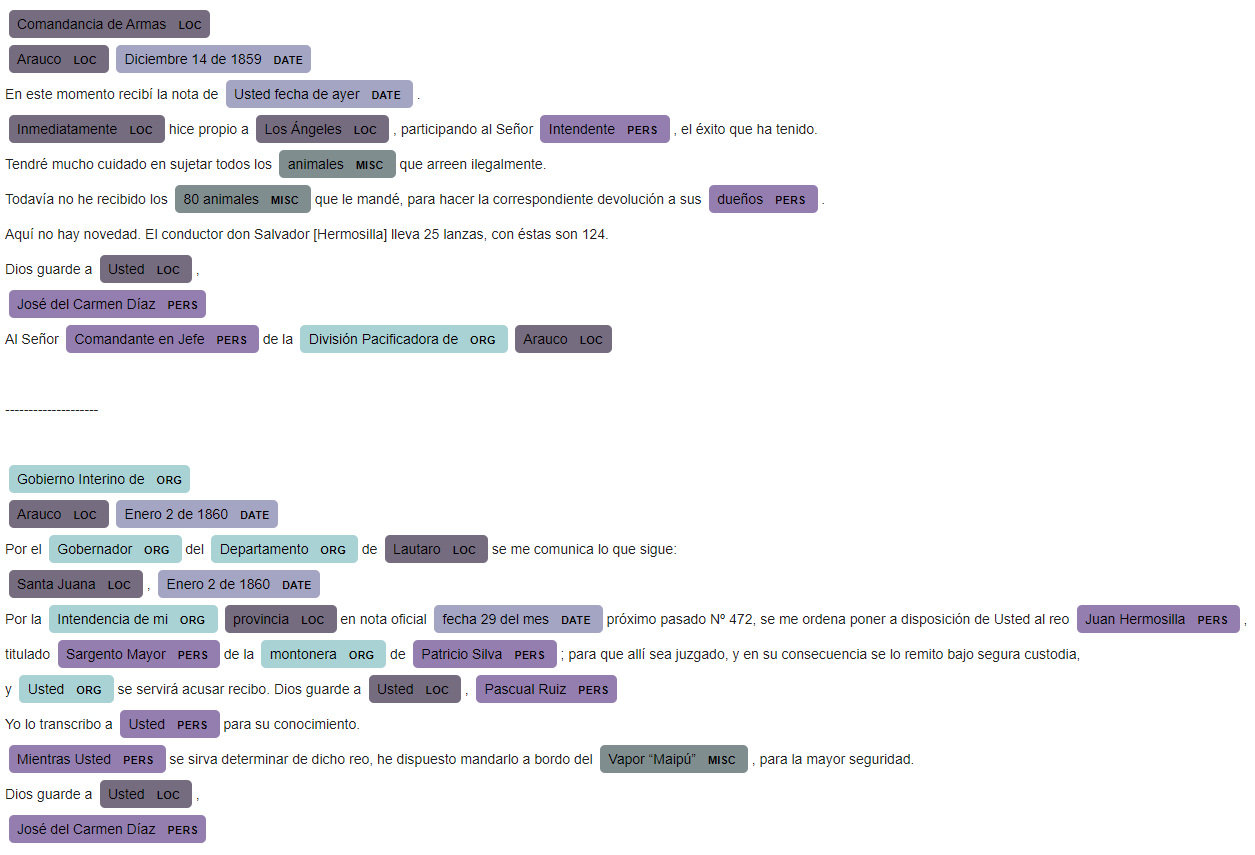
\includegraphics[width=0.8\textwidth]{annexes/img/k2_viz.png}
    \caption{Visualisation du modèle NER $\kappa_2$}
    \label{fig:k2_viz}
\end{figure}

\begin{figure}
    \centering
    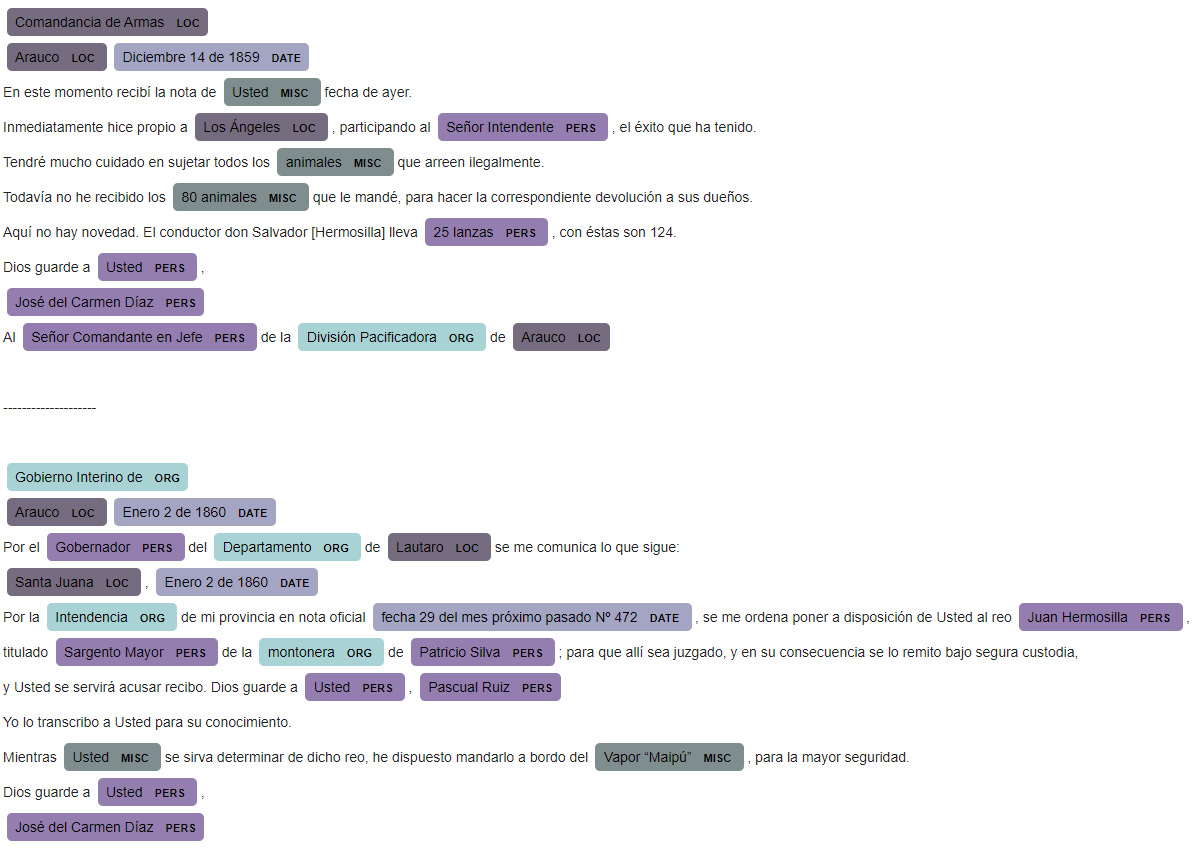
\includegraphics[width=0.8\textwidth]{annexes/img/k6_viz.png}
    \caption{Visualisation du modèle NER $\kappa_6$}
    \label{fig:k6_viz}
\end{figure}

\chapter{Modélisation d'entité XML-TEI à partir d'une requête SPARQL}
\chaptermark{Modélisation d'entité XML-TEI}

\begin{listing}[h]
	        \begin{minted}{xml}
<person xml:id="Q4233309" xml:base="https://viaf.org/viaf/534145858091523021888" xml:lang="en" sex="1.0">
  <persname>Cornelio Saavedra Rodríguez</persname>
  <birth when-iso="1821-01-01">1 de enero de 1821</birth>
  <death when-iso="1891-04-07">7 de abril de 1891</death>
  <note type="description">Chilean general</note>
</person>
	        \end{minted}
        	\caption{Structuration du <person> au sein du <particDesc>}
        	\label{code:ent_pers}
\end{listing}

\begin{listing}[h]
	        \begin{minted}{xml}
<place xml:id="Q33986" xml:base="https://www.geonames.org/3868626" xml:lang="en" type="city_in_Chile">
  <placename>Valparaíso</placename>
  <region>Valparaíso</region>
  <country>Chile</country>
  <geo>-71.619722222 -33.046111111</geo>
  <note type="description">city in Chile</note>
</place>
	        \end{minted}
        	\caption{Structuration du <place> au sein du <settingDesc>}
        	\label{code:ent_loc}
\end{listing}